%%%%% Magnetisches Feld %%%%%
%% #1 Beweis für die Existenz %%


%Some sample text to be displayed above the first subsection

%\subsection{Prinzip}

%Ein Zyklotron besteht aus Zwei hohlen, halbzylindrischen und Duanden an denen eine Spannung mit unterschiedlichem Vorzeichen anliegt, und darüber bzw. darunter liegende Magneten, die ein homogenes Magnetfeld erzeugen. Zudem gibt es einen Einlass und einen Auslass für Teilchen.

%\begin{wrapfigure}{r}{0.4\textwidth} \label{Zyklo}
%
%	\vspace{-10pt}
%	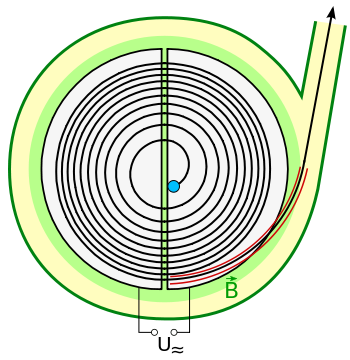
\includegraphics[width=0.35\textwidth]{Zyklotron_Prinzipskizze02.png}
%	\vspace{-13pt}
%	\caption{Prinzipskizze eines Zyklotrons}
%	\vspace{-5pt}	
%	
%\end{wrapfigure}

%\subsubsection{Anwendung}

% Some Formula:

%\begin{equation}
%	x= \frac{y \cdot 13 \pi z}
%			{\cos \alpha}
%\end{equation}

%%%%%%%%%%%%%%%%%%%%%%%
% Eigentlicher Beginn %
%%%%%%%%%%%%%%%%%%%%%%%

\subsection{Ferromagnetisches Metall}

Ein magnetisches Feld wird im klassischsten Sinne ausgelöst, wenn ein ferromagnetisches Metall \glqq magnetisiert\grqq{} wird, was heißt, dass sich sogenannte Elementarmagnete ausrichten.\footnote{Siehe: \url{https://de.wikipedia.org/wiki/Elementarmagnet}}


\subsection{Elektromagnet}

Jegliche Leiter, auch nicht-ferromagnetischer Natur, lösen ein magnetisches Feld aus, wenn Strom durch sie fließt.

Wenn Strom (also Elektronen, die kleinste Einheit der negativen Ladung) durch einen Leiter fließt, ergibt sich ein magnetisches Feld dessen Ausrichtung gemäß verschiedener Handregeln erfolgt. Siehe dazu \referenz{subsec:Faustregel}.


\subsection{Erdmagnetfeld}

Auch von der Erde geht ein magnetisches Feld aus, welches z.B. für Kompanten genutzt wird.

